\documentclass{article}

\usepackage[margin=1in]{geometry}
\usepackage{amssymb, amssymb, amsthm}
\usepackage{enumitem}
\usepackage{courier}
\usepackage{listings}
\usepackage{graphicx}
\usepackage{fancyvrb}
\usepackage{color}
\usepackage{hyperref}
\lstset
{
    language=Python,
    numbers=left,
    stepnumber=1,
    showstringspaces=false,
    tabsize=4,
    breaklines=true,
    breakatwhitespace=false,
}

\begin{document}
\pagenumbering{gobble}

\begin{flushright}
Keegan Dahm \\
CYBER W207 \\
Lab 3
\end{flushright}

\begin{enumerate}[start=1]
\item % 1
    The training data had 126 columns. PCA quickly caught up, and was able to explain 90\% of data variance with only 30 components, which can significantly reduce model training costs.
    
    \begin{center}
    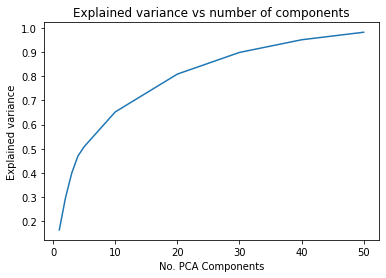
\includegraphics[width=5cm]{part1.0.png}
    \end{center}

\item % 2
    For this, I generated a second graph, where non-poisonous samples are semi-transparent. This helps show the overlap between the two categories after 2-component PCA.
    
    \begin{center}
    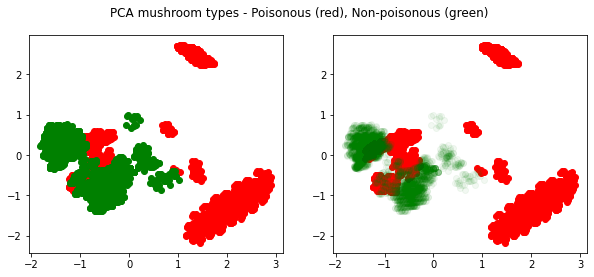
\includegraphics[width=10cm]{part2.0.png}
    \end{center}
    
    As this chart shows, some poisonous clusters end up distinctly separated from the rest and are easily distinguishable, while some clusters overlap, and would need more components to tell apart.
    
\item % 3
    

\end{enumerate}

\end{document}
